% Options for packages loaded elsewhere
\PassOptionsToPackage{unicode}{hyperref}
\PassOptionsToPackage{hyphens}{url}
\PassOptionsToPackage{dvipsnames,svgnames,x11names}{xcolor}
%
\documentclass[
  12pt,
]{article}
\usepackage{amsmath,amssymb}
\usepackage{iftex}
\ifPDFTeX
  \usepackage[T1]{fontenc}
  \usepackage[utf8]{inputenc}
  \usepackage{textcomp} % provide euro and other symbols
\else % if luatex or xetex
  \usepackage{unicode-math} % this also loads fontspec
  \defaultfontfeatures{Scale=MatchLowercase}
  \defaultfontfeatures[\rmfamily]{Ligatures=TeX,Scale=1}
\fi
\usepackage{lmodern}
\ifPDFTeX\else
  % xetex/luatex font selection
\fi
% Use upquote if available, for straight quotes in verbatim environments
\IfFileExists{upquote.sty}{\usepackage{upquote}}{}
\IfFileExists{microtype.sty}{% use microtype if available
  \usepackage[]{microtype}
  \UseMicrotypeSet[protrusion]{basicmath} % disable protrusion for tt fonts
}{}
\makeatletter
\@ifundefined{KOMAClassName}{% if non-KOMA class
  \IfFileExists{parskip.sty}{%
    \usepackage{parskip}
  }{% else
    \setlength{\parindent}{0pt}
    \setlength{\parskip}{6pt plus 2pt minus 1pt}}
}{% if KOMA class
  \KOMAoptions{parskip=half}}
\makeatother
\usepackage{xcolor}
\usepackage[margin=0.75in]{geometry}
\usepackage{graphicx}
\makeatletter
\def\maxwidth{\ifdim\Gin@nat@width>\linewidth\linewidth\else\Gin@nat@width\fi}
\def\maxheight{\ifdim\Gin@nat@height>\textheight\textheight\else\Gin@nat@height\fi}
\makeatother
% Scale images if necessary, so that they will not overflow the page
% margins by default, and it is still possible to overwrite the defaults
% using explicit options in \includegraphics[width, height, ...]{}
\setkeys{Gin}{width=\maxwidth,height=\maxheight,keepaspectratio}
% Set default figure placement to htbp
\makeatletter
\def\fps@figure{htbp}
\makeatother
\setlength{\emergencystretch}{3em} % prevent overfull lines
\providecommand{\tightlist}{%
  \setlength{\itemsep}{0pt}\setlength{\parskip}{0pt}}
\setcounter{secnumdepth}{-\maxdimen} % remove section numbering
\usepackage{fancyhdr}
\pagestyle{fancy}
\fancyfoot{}
\usepackage[default]{sourcesanspro}
\usepackage{parskip}
\usepackage{geometry}
\usepackage{caption}
\usepackage{xcolor}
\definecolor{green}{RGB}{0,102,0}
\definecolor{blue}{RGB}{0, 0, 139}
\definecolor{darkcerulean}{rgb}{0.03, 0.27, 0.49}
\definecolor{darkmidnightblue}{rgb}{0.0, 0.2, 0.4}
\AtBeginDocument{\let\maketitle\relax}
\usepackage[none]{hyphenat}
\usepackage[document]{ragged2e}
\usepackage{graphicx}
\usepackage{geometry}
\usepackage{sectsty}\allsectionsfont{\raggedright}
\usepackage{sectsty}\sectionfont{\centering\color{darkmidnightblue}}
\usepackage{sectsty}\subsectionfont{\centering\color{darkmidnightblue}}
\usepackage{titlesec}
\usepackage{longtable}
\usepackage{tabu}
\usepackage{wrapfig}
\usepackage[export]{adjustbox}
\titlespacing{\section}{0pt}{24pt plus 2pt minus 1pt}{0pt plus 1pt minus 1pt}
\titlespacing{\subsection}{0pt}{12pt plus 2pt minus 1pt}{0pt plus 1pt minus 1pt}
\titlespacing{\subsubsection}{0pt}{12pt plus 2pt minus 1pt}{0pt plus 1pt minus 1pt}
\usepackage{pdflscape}
\newcommand{\blandscape}{\begin{landscape}}
\newcommand{\elandscape}{\end{landscape}}
\usepackage{floatrow}
\DeclareFloatSeparators{mysep}{\hskip-94em}
\floatsetup[figure]{capposition=beside,capbesidesep=mysep,capbesideposition={right, center}}
\ifLuaTeX
  \usepackage{selnolig}  % disable illegal ligatures
\fi
\usepackage{bookmark}
\IfFileExists{xurl.sty}{\usepackage{xurl}}{} % add URL line breaks if available
\urlstyle{same}
\hypersetup{
  pdftitle={HerbVar Newsletter, January 2025},
  pdfauthor={The HerbVar Steeting Committee},
  colorlinks=true,
  linkcolor={blue},
  filecolor={Maroon},
  citecolor={Blue},
  urlcolor={blue},
  pdfcreator={LaTeX via pandoc}}

\title{HerbVar Newsletter, January 2025}
\author{The HerbVar Steeting Committee}
\date{2025-01-17}

\begin{document}
\maketitle

\thispagestyle{empty}

Dear HerbVar members,

Greetings and Happy New Year! The HV Steering Committee has spent the
last year building the infrastructure to bring our network into its next
stage of collaboration! We are writing with four big updates:

\begin{enumerate}
\def\labelenumi{\arabic{enumi}.}
\tightlist
\item
  \textbf{\hyperref[manual]{New HerbVar Manual and collaborative GitHub
  organization}}\\
\item
  \textbf{\hyperref[help]{Help Wanted: Data on damage to reproductive
  structures}}\\
\item
  \textbf{\hyperref[wg1]{Upate on new papers and Working Groups}}\\
\item
  \textbf{\hyperref[wg2]{Call for Proposals: New HerbVar Working
  Groups}}
\end{enumerate}

\subsection{New HerbVar Manual and collaborative GitHub
organization}\label{manual}

Emilio Bruna has led an amazing effort to bring cutting edge
collaboration techniques to HV. As part of this, we have migrated our
collaborative infrastructure from Google Drive to a collaborative GitHub
Organization: \url{https://github.com/HerbVar-Network}. This will
facilitate sharing data and code among new Working Groups. It includes
automated scripts for downloading and wrangling HV data. As part of
this, we have also collected all of our diverse materials (protocols,
guides, and policies) into a single, centralized HV Manual, which can be
viewed via our GitHub Organization as an
\href{https://herbvar-network.github.io/herbvar_manual/}{HTML book} or a
\href{https://herbvar-network.github.io/herbvar_manual/herbvar-manual.pdf}{PDF}.
You can contribute to the manual by suggesting edits through the
\href{https://github.com/HerbVar-Network/herbvar_manual}{GitHub
repository for the manual}.

\begin{figure}
\centering

\includegraphics[width=2.08333in,height=\textheight]{images_2025-01/HV_manual_cover.png}
\caption{The cover of the HV Manual}
\end{figure}

The manual is also citable - please cite it if you use or build off of a
HV protocol:

\begin{quote}
``HerbVar Steering Committee (2024). HerbVar: Project Manual and Field
protocols (v0.9.0). Zenodo.
\url{https://doi.org/10.5281/zenodo.14232308}.''
\end{quote}

Thanks to Emilio Bruna for helping to make HV a leader in collaborative
ecological networks!

\subsection{Help Wanted: Data on damage to reproductive
structures}\label{help}

Please consider participating in our current sampling objectives! Our
most pressing need is data from reproductive damage surveys. We
currently have about 70 reproductive surveys. The preliminary results
are very exciting. We think that the reproductive paper will be as
important as our Science paper, but we need bigger sample sizes to be
able to test big ideas. So we encourage everyone to take a few days to
collect and submit data using our Reproductive Protocol, which has been
polished recently and included in the
\href{https://herbvar-network.github.io/herbvar_manual/protocols/repro_damage.html}{HV
Manual}. Susan Whitehead is planning to lead the Reproductive Damage
Working Group.

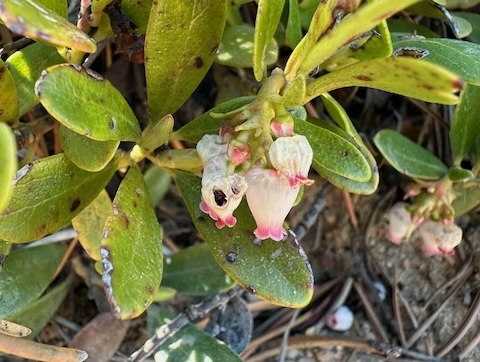
\includegraphics[width=2.08333in,height=\textheight]{images_2025-01/IMG_3986.jpeg}

Our additional objectives include data from our focal families and focal
species. And, as always, we are willing to accept any data following an
HV protocol with any plant species. Data submission helps us grow our
public database for the benefit of the whole field. Of course, surveys
with species that aren't currently part of a major sampling objective
may take longer to lead to a Working Group publication, unless you
decide to lead one! See below.

\subsection{Upate on new papers and Working Groups}\label{wg1}

We are excited to announce the initiation of several new HV Working
Groups. The list of Working Groups can be found
\href{https://herbvar.org/workingGroups.html}{here}. The Spatial Pattern
Working Group (led by Will Wetzel) will include as co-authors all HV
members who contributed data (Site PIs), including everyone who
contributed data to our Science paper. The Focal Family Working Group
(led by Ivalú Cacho) will include all HV Site PIs who contributed focal
family data. An Education Working Group (led by Nora Underwood) has
started collecting materials related to teaching about biological
variability. Stay tuned to hear more from the leaders of these Working
Groups.

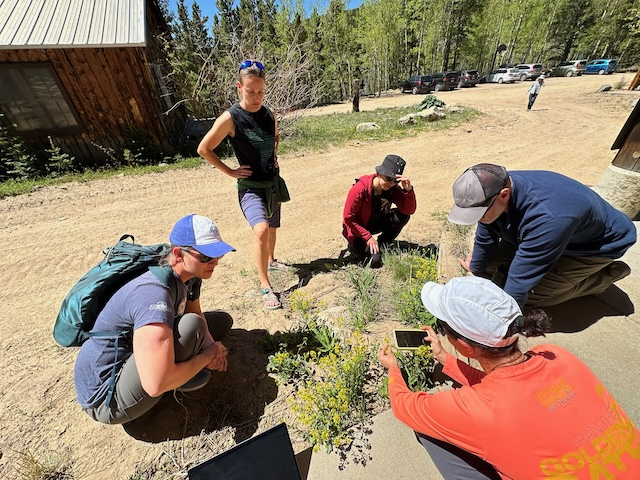
\includegraphics[width=2.08333in,height=\textheight]{images_2025-01/IMG_3997.jpeg}

\subsection{Call for Proposals: New HerbVar Working Groups}\label{wg2}

We are now open to considering proposals for new HV Working Groups from
any HV member. This includes Working Groups that use existing data or
Working Groups that develop and circulate new, add-on data collection
protocols. If you are interested in leading a Working Group, please
review the relevant section of the HV Manual, which describes the
\href{https://herbvar-network.github.io/herbvar_manual/collaboration/working-group-pubs.html}{process
for proposing and initiating a Working Group}.

Thank you so much for being part of HerbVar!

Warm regards,\\
The HV Steering Committee

Karen Abbott\\
Emilio Bruna\\
Ivalú Cacho\\
Lee Dyer\\
Phil Hahn\\
Brian Inouye\\
Nora Underwood\\
Will Wetzel\\
Susan Whitehead

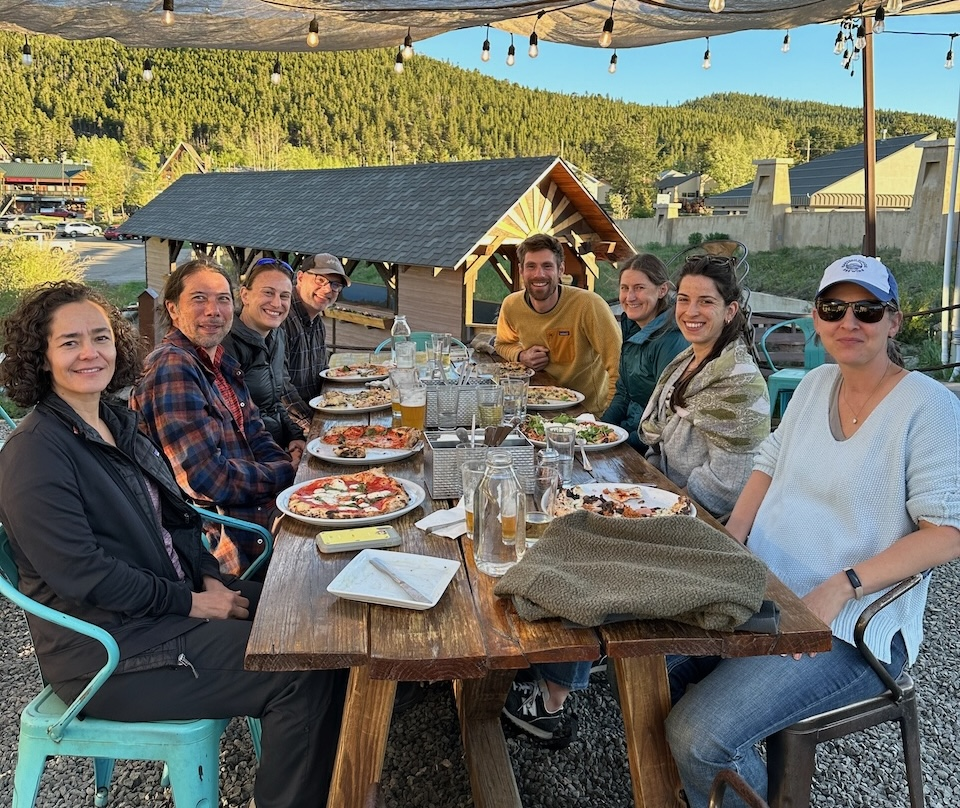
\includegraphics[width=4.16667in,height=\textheight]{images_2025-01/IMG_3994.jpeg}

\begin{center}\rule{0.5\linewidth}{0.5pt}\end{center}

\subsection{Stay in touch}\label{stay-in-touch}

You can read this and all prior newsletters on our
\href{https://herbvar.org/}{website}, where you can also get updates on
ongoing projects and download the most recent HerbVar
\href{https://herbvar.org/products.html}{publications}.

\end{document}
